%************************************************
\section{Validation and Performance Evaluation}\label{ch:validation}
%************************************************

% TODO:
% https://abc4trust.eu/download/D4.2%20Final%20Reference%20Implementation.pdf
% Comparar con página 44

This section describes the deployment of three testing scenarios with different hardware capabilities. A laptop, a standalone Raspberry Pi 3 (RPi3), and an Omega2 IoT device with the Raspberry Pi 3 as the delegation server. The scenarios aim to measure and compare the results to determine whether the proposed solution runs as expected and it is feasible.

\subsection{Testbed description}

%First, we shall describe the example Attribute Based Credential system in use. Then, the hardware we will use in our benchmarking.

%\subsubsection{P2ABCE setting}

To verify the correct execution of the \textit{IoT smart card}, the test is based on the ABC system from the tutorial in the P2ABCE Wiki\footnote{\url{https://github.com/p2abcengine/p2abcengine/wiki/}}. It consists on a soccer club, which wishes to issue VIP-tickets for a match. The VIP-member number in the ticket is inspectable for a lottery, ie. after the game, a random presentation token is inspected and the winning member is notified.

First, the \textbf{setup} phase takes place, where several artifacts are generated and distributed to the various P2ABCE entities. Next, a ticket credential containing the following attributes is \textbf{issued}:
\begin{Verbatim}[fontsize=\footnotesize]
First name: John	Member number: 23784638726	
Last name: Dow	  Matchday: 2013-08-07Z
Birthday: 1985-05-05Z
\end{Verbatim}

%During the \textbf{issuance}, a \textit{scope exclusive pseudonym} is established and the newly issued credential is bound to this pseudonym. This ensures that the ticket credential can not be used without the smart card.

Then a \textbf{presentation} is performed, where a \textit{presentation policy} from the verifier specifies that the member number is inspectable and a predicate which ensures that the matchday is in fact $2013-08-07Z$. This last part ensures that a ticket issued for another match can not be used. The policy also includes the nonce value for the proof's challenge.

\hfil

%\subsubsection{Execution environment}

First we will execute the test in our development laptop. After asserting that the services work as expected, we then proceed to run the test in a RPi3\footnote{\url{https://www.raspberrypi.org/products/raspberry-pi-3-model-b/}}, exactly like in the laptop. Finally, the PoC IoT smart card will be deployed in an Omega2\footnote{\url{https://docs.onion.io/omega2-docs/omega2.html}} and the delegation services in the RPi3.
%After each test, we checked that the issuing and proving were successful, in case a cryptographic error appeared in the implementation.
%A downside of using the Omega2 is the lack of hardware acceleration for cryptographic operations, unlike the MULTOS smart cards.

\hfil

The third scenario involves communications over TCP in a LAN. The RPi3 is connected over Ethernet to a switch with a WiFi access point. The Omega2 is connected over WiFi n to said AP. To test the possible network delays, $6000$ samples of APDU messages were taken from the test executions, and sent between the two devices, without handling the APDUs. The results show a mean of $14\mu s$ per byte sent, i.e. less than half a millisecond per APDU.



\subsection{Results}

After 20 executions for each scenario (laptop, RPi3, Omega2+RPi3), the time was measured for each REST call executed against the User Service in the delegation server, to later take the means to compare each step of the testbed. Because during a call to the User Service, the server may contact the \textit{IoT Smart Card}, the difference in times between the second and third scenario will show the performance of our IoT PoC.

It is worth noting that during the tests, the CPU usage showed that P2ABCE does not benefit from parallelization, therefore it only uses one of the four available cores in the laptop and Raspberry Pi 3.

%\paragraph{The setup}\hfil
\hfil

The IoT device does not intervene in the first step of the testbed, the setup, until the initialization of the new smart card, thus the times measured for each REST call in the second and third scenarios are practically identical as shown in Fig.~\ref{fig:setup:graph}. The laptop is about ten times faster than the Raspberry Pi 3. It is also noticeable that the setup step is only done once, and the highest time measured is less than two and a half seconds.

\begin{figure}[bth]
	\centering
	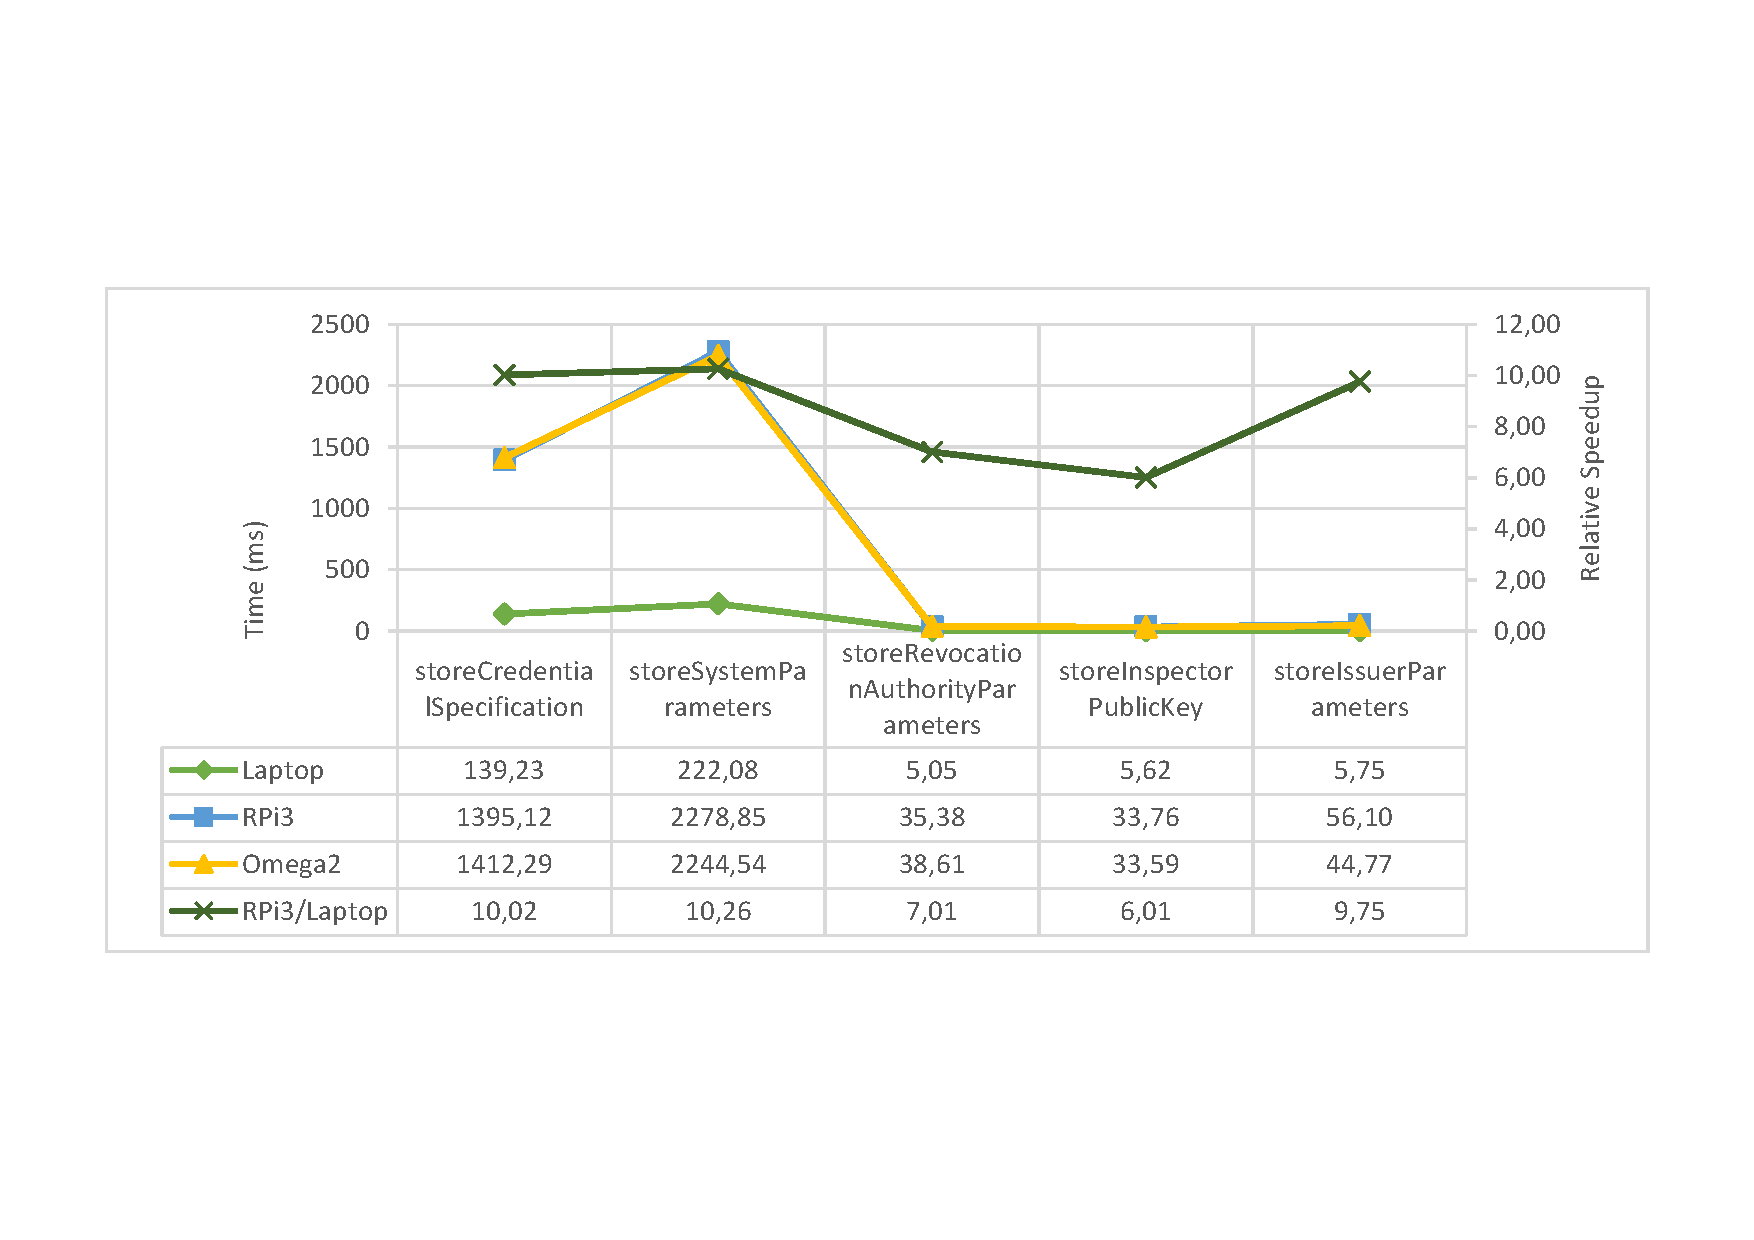
\includegraphics[width=\linewidth]{gfx/graphics/SetupGraphTable}
	\caption{Setup times (milliseconds) and relative speedup.}
	\label{fig:setup:graph}
\end{figure}

%\begin{figure}[bth]
%	\caption{Setup times (milliseconds). Comparison graph}
%	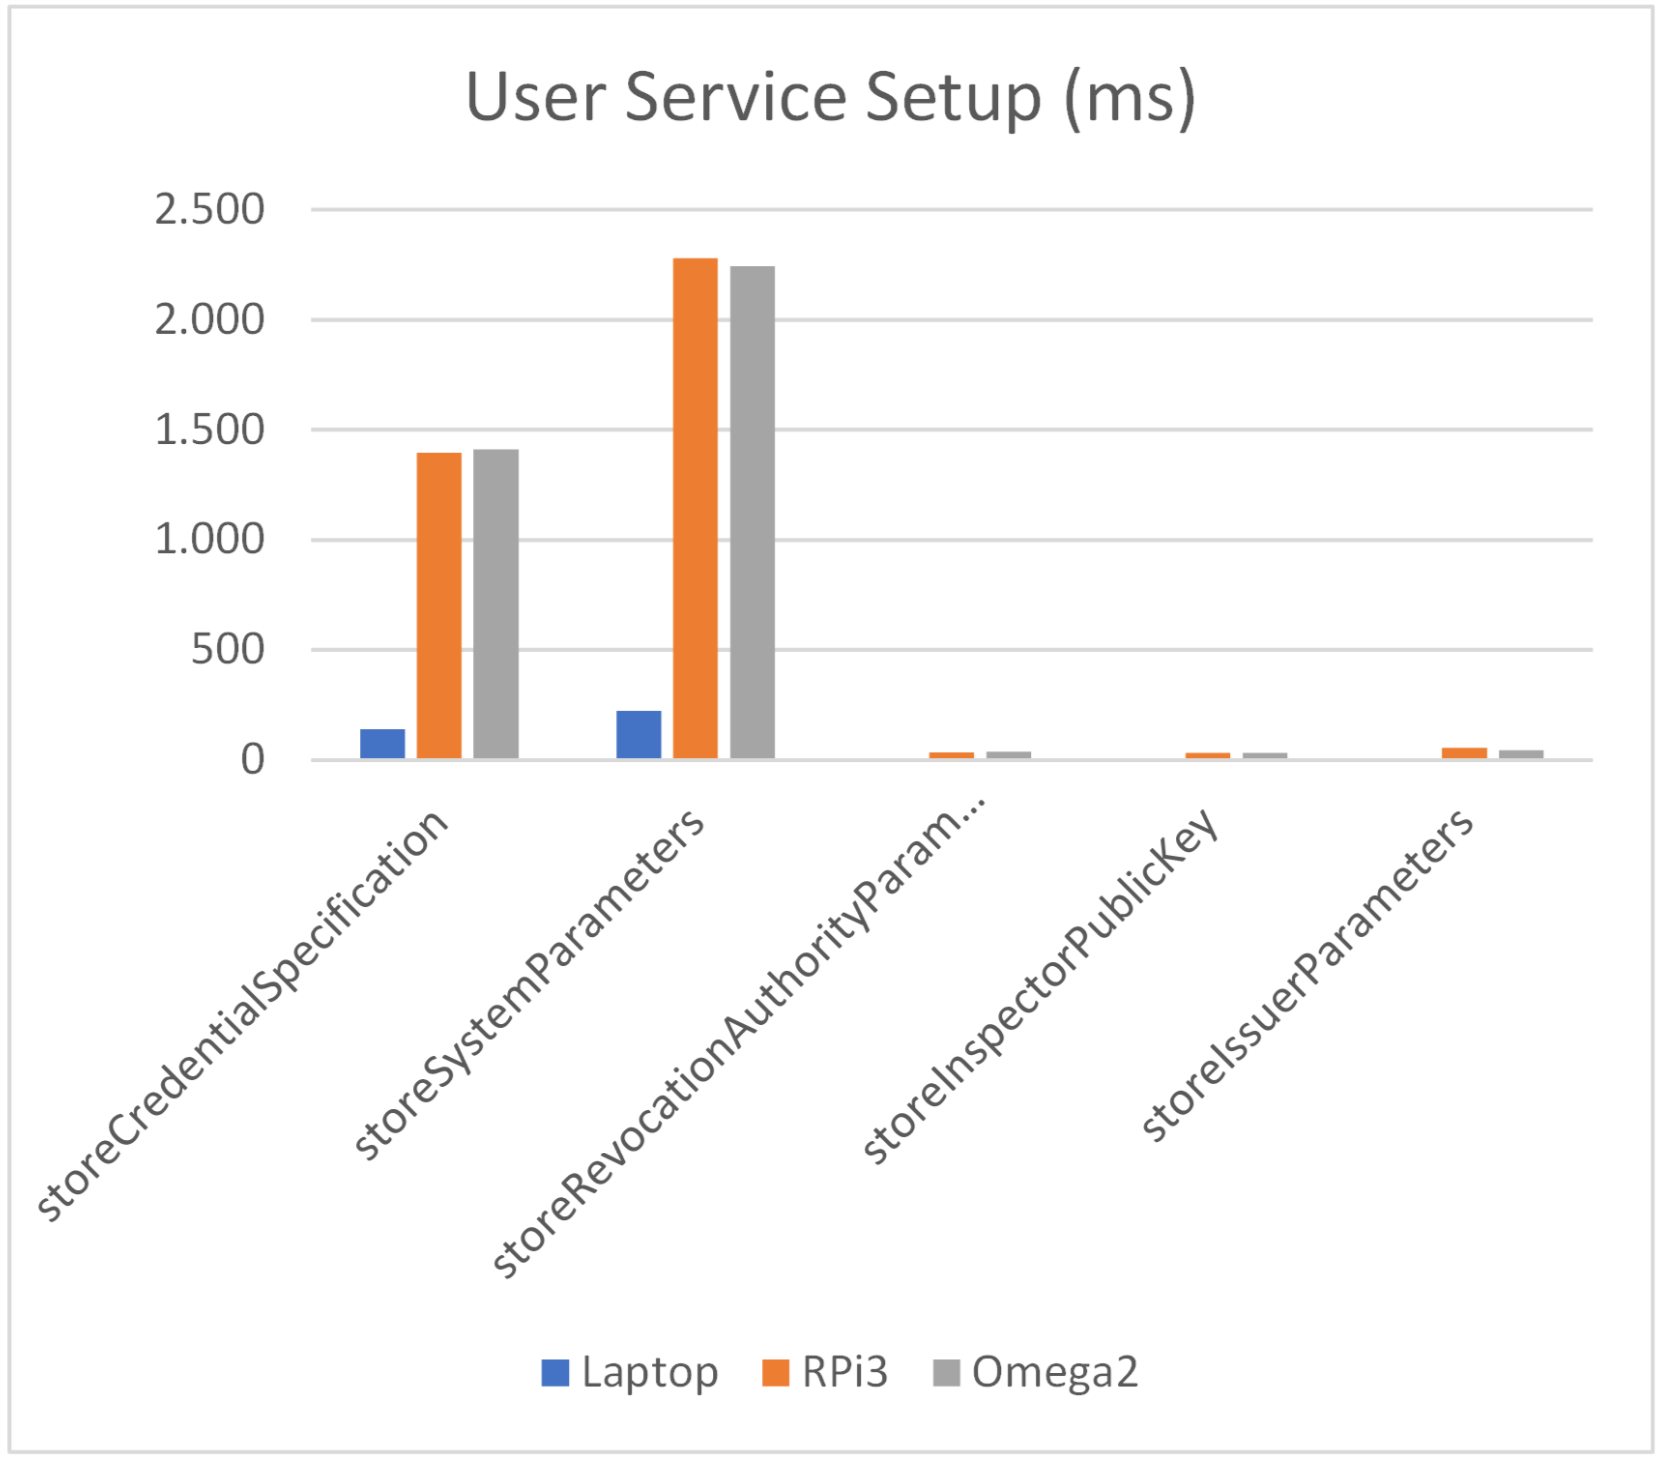
\includegraphics[width=0.8\linewidth]{gfx/graphics/setup}
%	\label{fig:setup:graph2}
%\end{figure}



%\paragraph{Creation of the smart card}\hfil
\hfil

The creation of a \texttt{SoftwareSmartcard} or a \texttt{HardwareSmartcard}, which actually uses the \texttt{IoT Smart Card}, differ in how the hardware version must copy to an external device the cryptographic information of the system, shared during the setup phase, as well as common smart card functionality, like the PIN, PUK, operation mode, etc. Figure~\ref{fig:createSmartCard:graph} shows this difference between the software versions of the laptop and RPi3, and the IoT version. This is a one time procedure per device.


\begin{figure}[bth]
	\centering
	\includegraphics[width=0.6\linewidth]{gfx/graphics/createSCGraph}
	\caption{Create smart card times (seconds).} 
	\label{fig:createSmartCard:graph} 
\end{figure}


%\begin{figure}[bth]
%	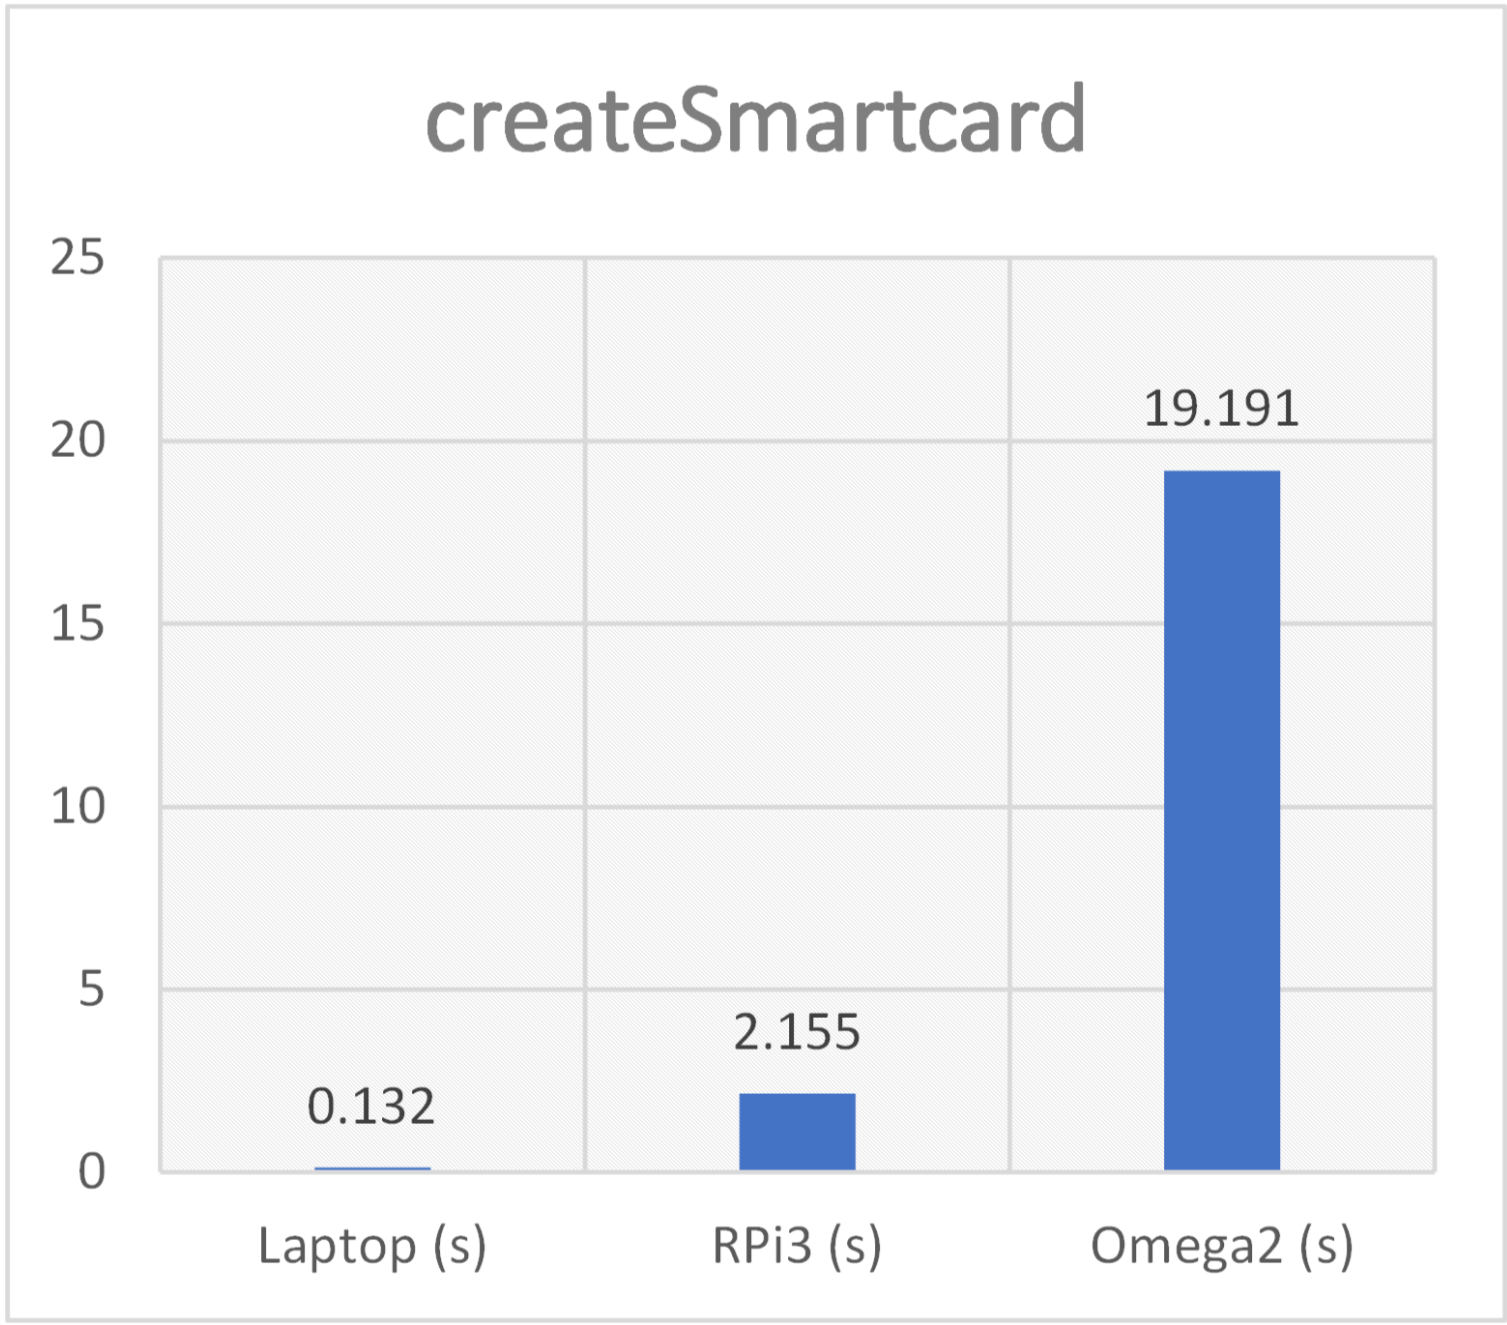
\includegraphics[width=0.8\linewidth]{gfx/graphics/createSC}
%	\caption{Create smart card times (seconds). Comparison graph}
%	\label{fig:createSmartCard:graph2}
%\end{figure}

As this is the first interaction between the RPi3 and the IoT smart card running in the Omega2, it is interesting to analyse the possible network delays. The process uses $30$ APDU Commands, and their respective Responses, with a total of $1109$ bytes. From the network benchmark, the delay in the transmission is around 15 and 20 ms, negligible compared to the total operation time.


%\paragraph{Issuance of the credential}\hfil
\hfil

The results for the Issuance step of the credential with 5 attributes and key sizes of 1024 bits is shown in Figure~\ref{fig:issuance:graph}. The process is performed with three REST calls to the User Service, corresponding to the multi-step Idemix credential issuance and identity to use selection.  The results shows the times for each call in each device, and the increase of time from the RPi3 to the Omega2 case highlights the difference of processing power between the devices, where the first one makes use of the Java implemented smart card, and the Omega 2 runs the IoT PoC smart card.



%The three delegation steps and the REST method called are:
%
%\begin{itemize}
%	\item First issuance protocol step:\\\texttt{/issuanceProtocolStep}
%	\item Second issuance protocol step (end of first step for the User): \texttt{/issuanceProtocolStepUi}
%	\item Third issuance protocol step (second step for the User): \texttt{/issuanceProtocolStep}
%\end{itemize}



%\begin{figure}[bth]
%	\begin{center}
%		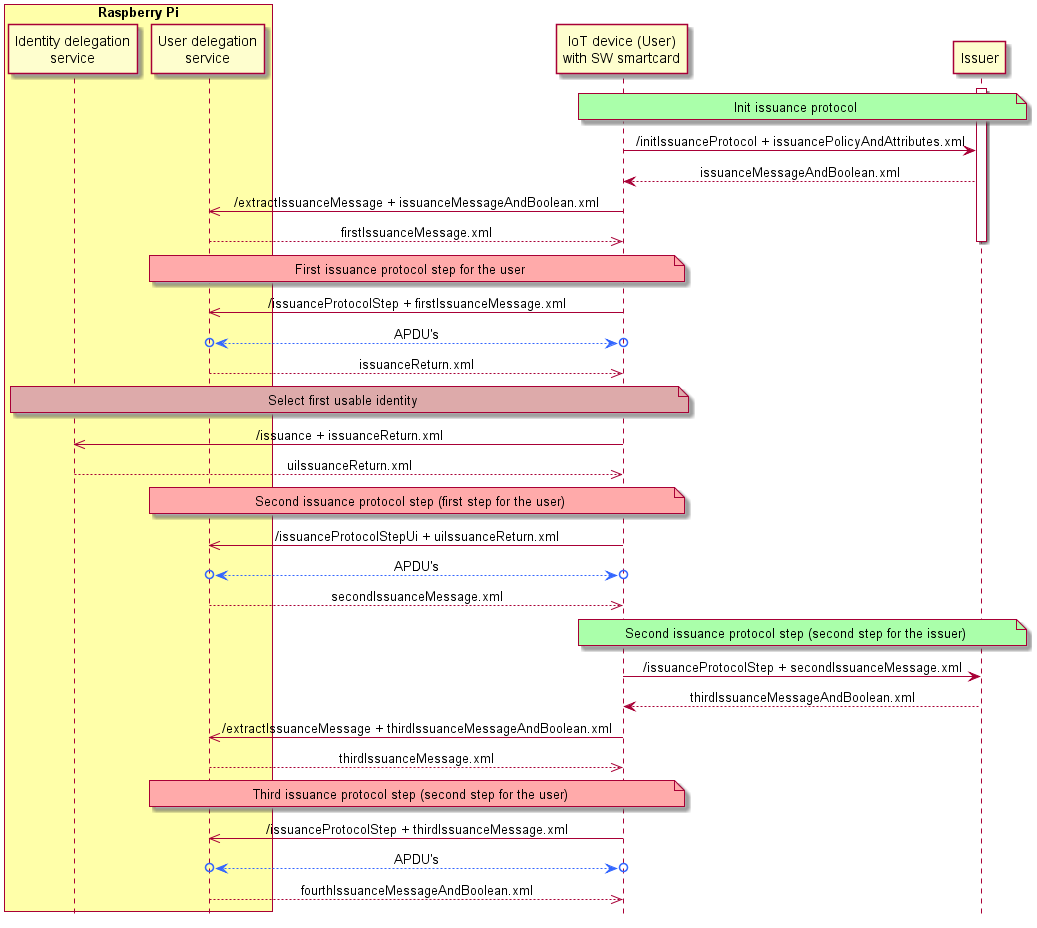
\includegraphics[width=\linewidth]{gfx/UML/IssuanceInteraction}
%	\end{center}
%	\caption{Issuance interaction.}
%	\label{fig:IssuanceInteraction}
%\end{figure}



The three REST calls to the delegation service involved APDU Dialogues with the IoT smart card, with $45$ APDU Commands in total, $3197$ bytes exchanged, that would have introduced a latency of only 45ms from the network.


\begin{figure}[bth]
	\centering
	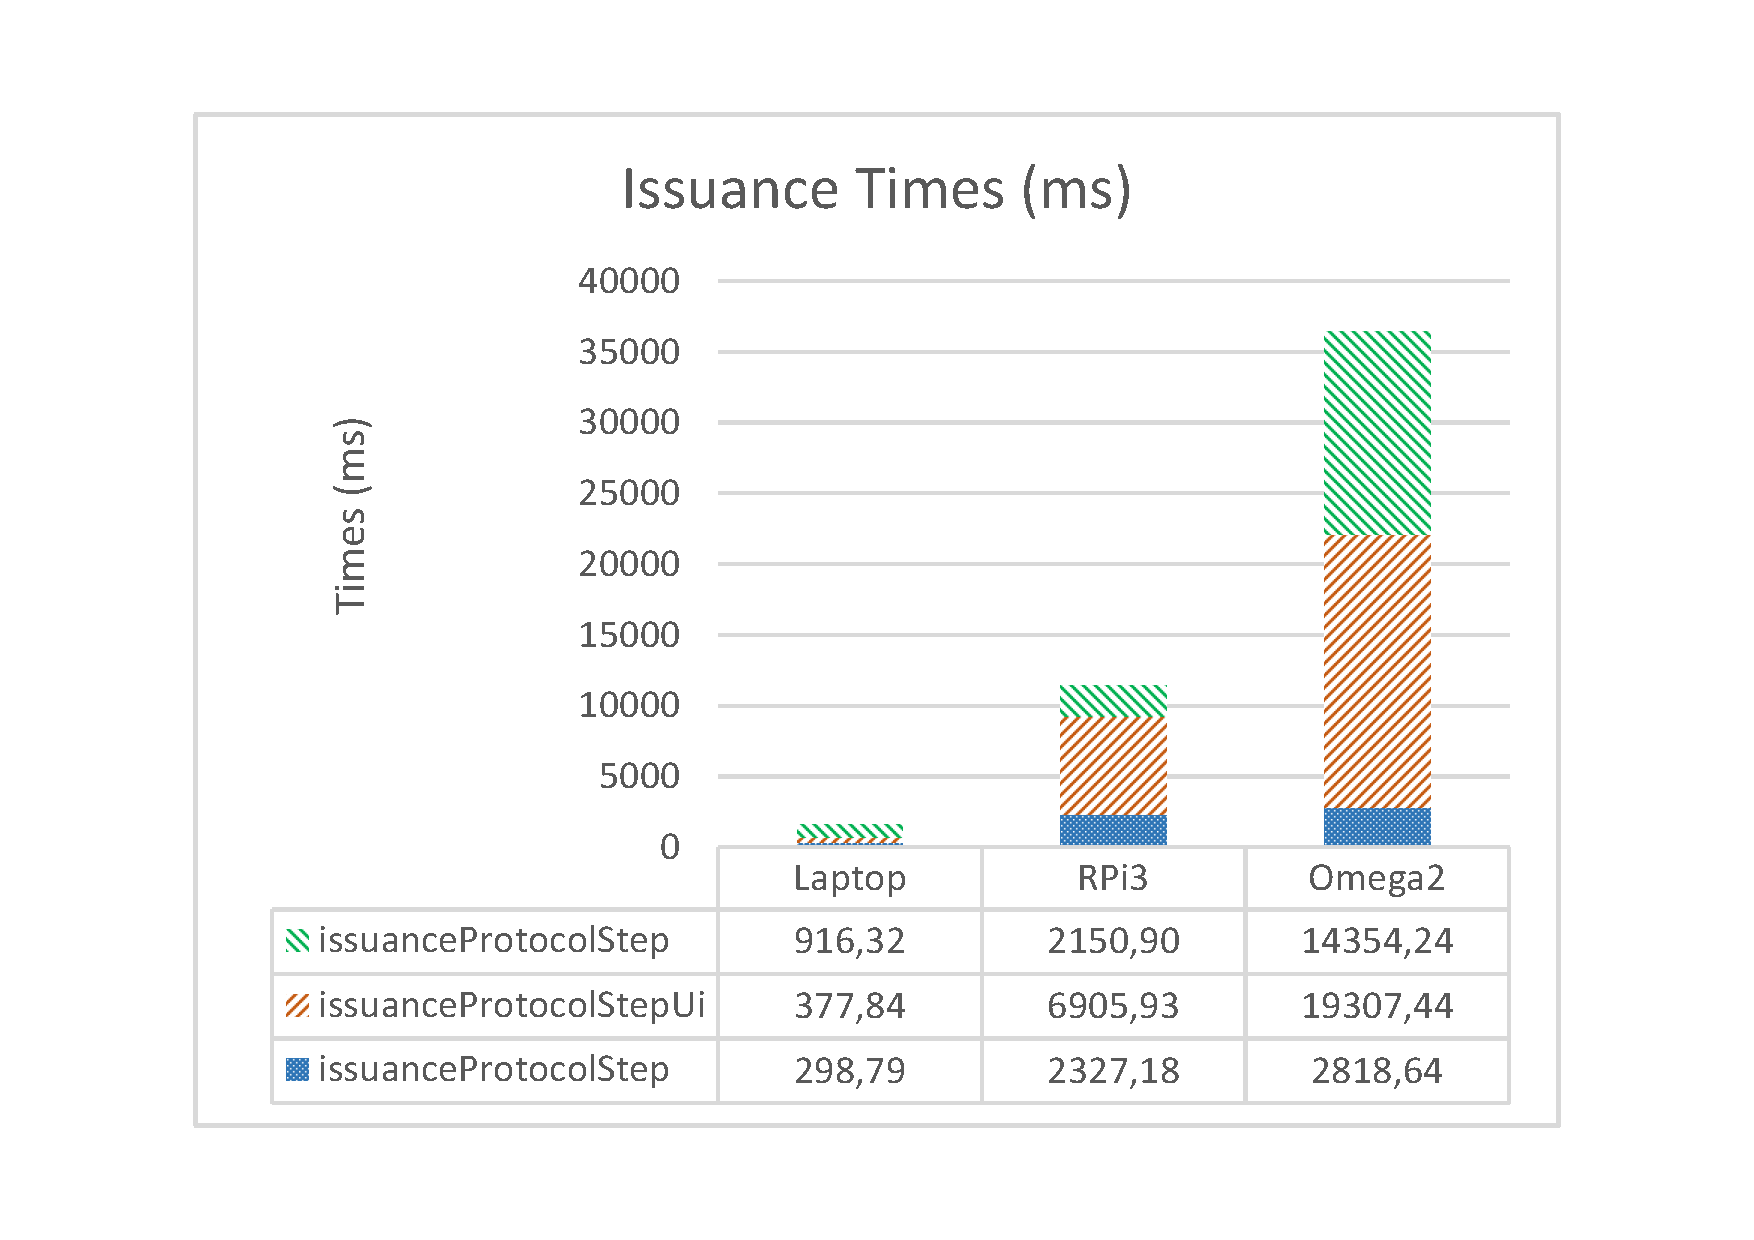
\includegraphics[width=0.8\linewidth]{gfx/graphics/IssuanceGraphTable}
	\caption{Issuance times (milliseconds)}% and relative speedup.}
	\label{fig:issuance:graph}
\end{figure}

%\begin{figure}[bth]
%	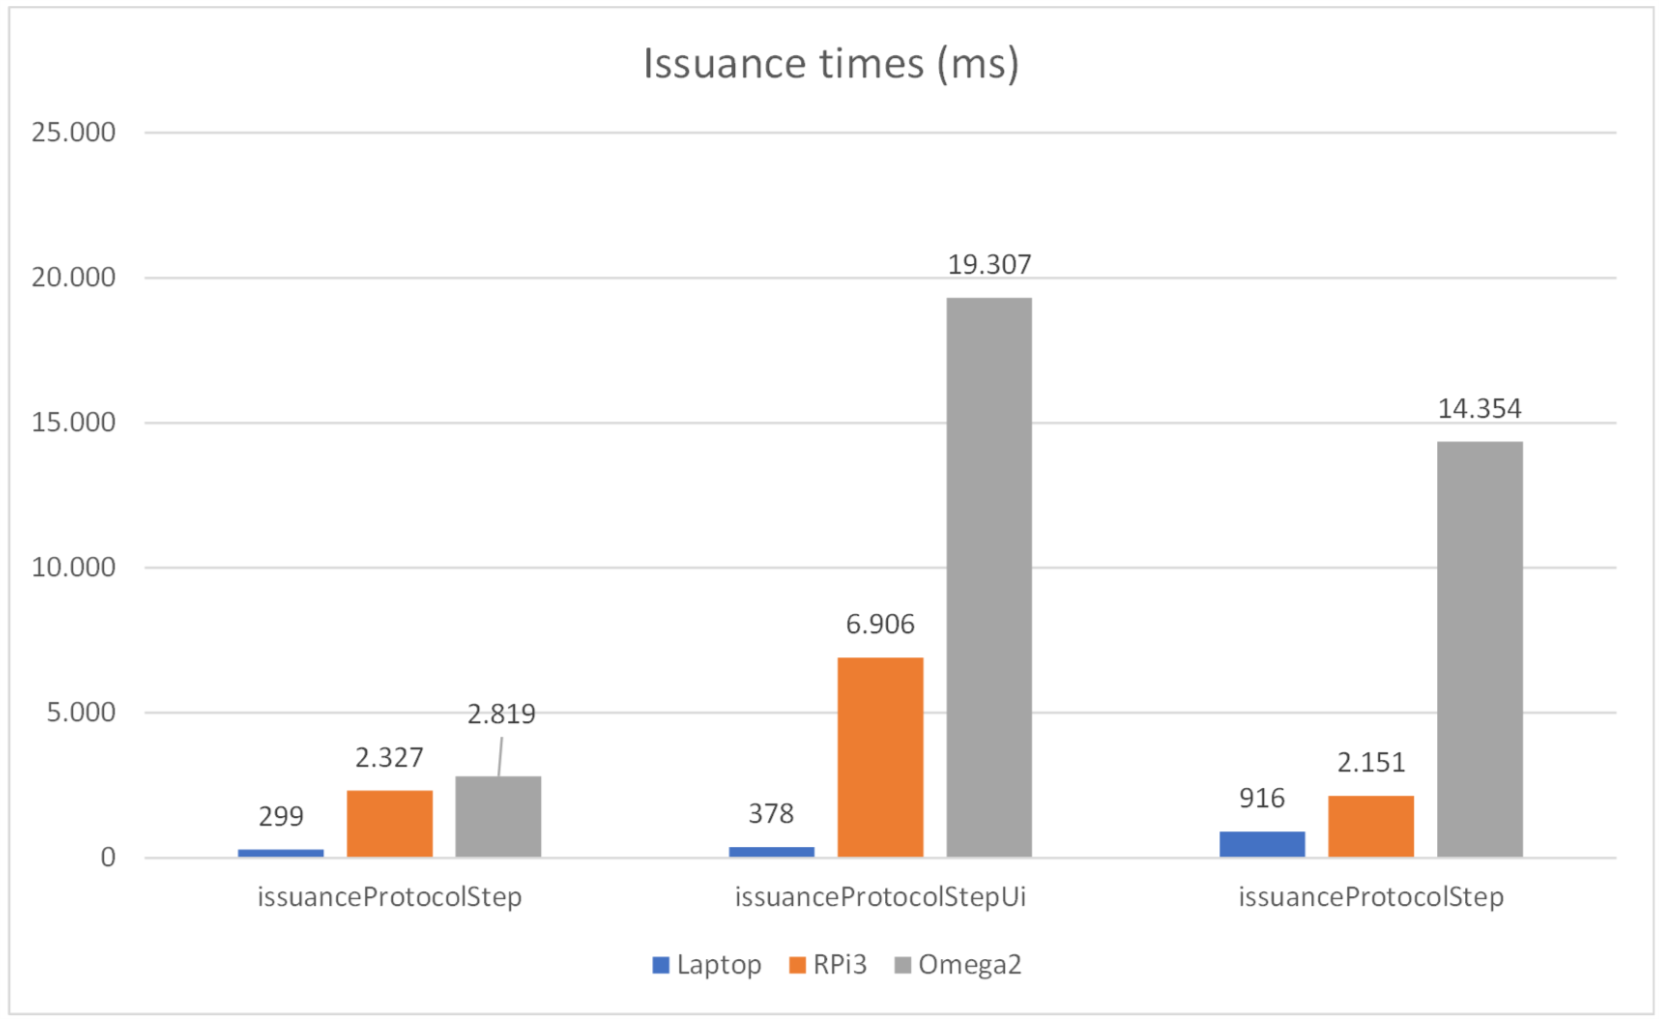
\includegraphics[width=\linewidth]{gfx/graphics/issuance}
%	\caption{Issuance times (milliseconds). Comparison graph}
%	\label{fig:issuance:graph2}
%\end{figure}



%\paragraph{Presentation token}\hfil
\hfil

The final step of the test involves a Proving or Presentation in P2ABCE, where the Verifier sends the User a Presentation Policy, and the User answers with the Presentation Token, without more steps from the User. To ensure that all the process was successful, it was enough to check from the Verifier and the Inspector perspectives that every Token generated was valid.

%\begin{figure}[bth]
%	\begin{center}
%		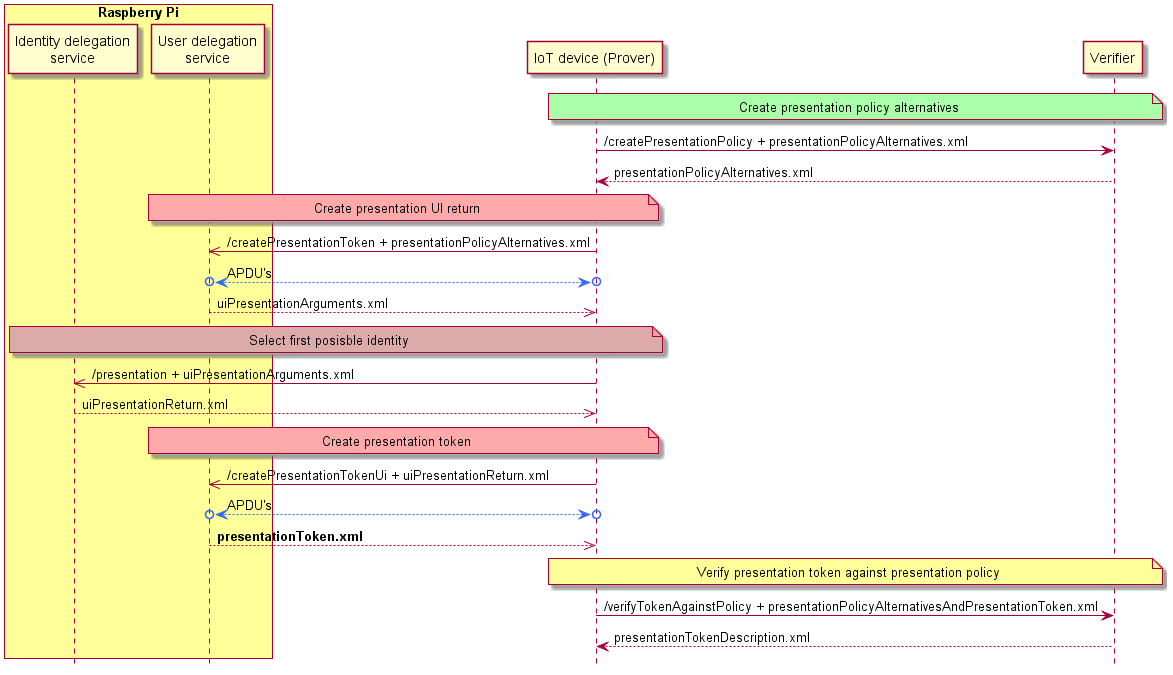
\includegraphics[width=\linewidth]{gfx/UML/ProvingInteraction}
%	\end{center}
%	\caption{Proving interaction.}
%	\label{fig:ProvingInteraction}
%\end{figure}

As shown in Fig.~\ref{fig:proving:graph}, there is a correlation between the cryptographic work the IoT smart card must perform, and the increase of time measured from the RPi3 to the Omega2 cases. 
The APDU Dialogue involved $28$ APDUs, with $1939$ bytes, about only $27$ms of delay from the network.

%The $20$ APDU Commands in the first call make the IoT deployment almost $8$ times slower than the Raspberry Pi 3; but with only $8$ APDU Commands, the second one is less than $1.5$ times slower.

%Nonetheless, it's significant the difference in performance between the laptop and the Raspberry Pi 3 in the last REST call, more than $40$ times slower, even using the \textit{SoftwareSmartcard} in the RPi3.

\begin{figure}[bth]
	\centering
	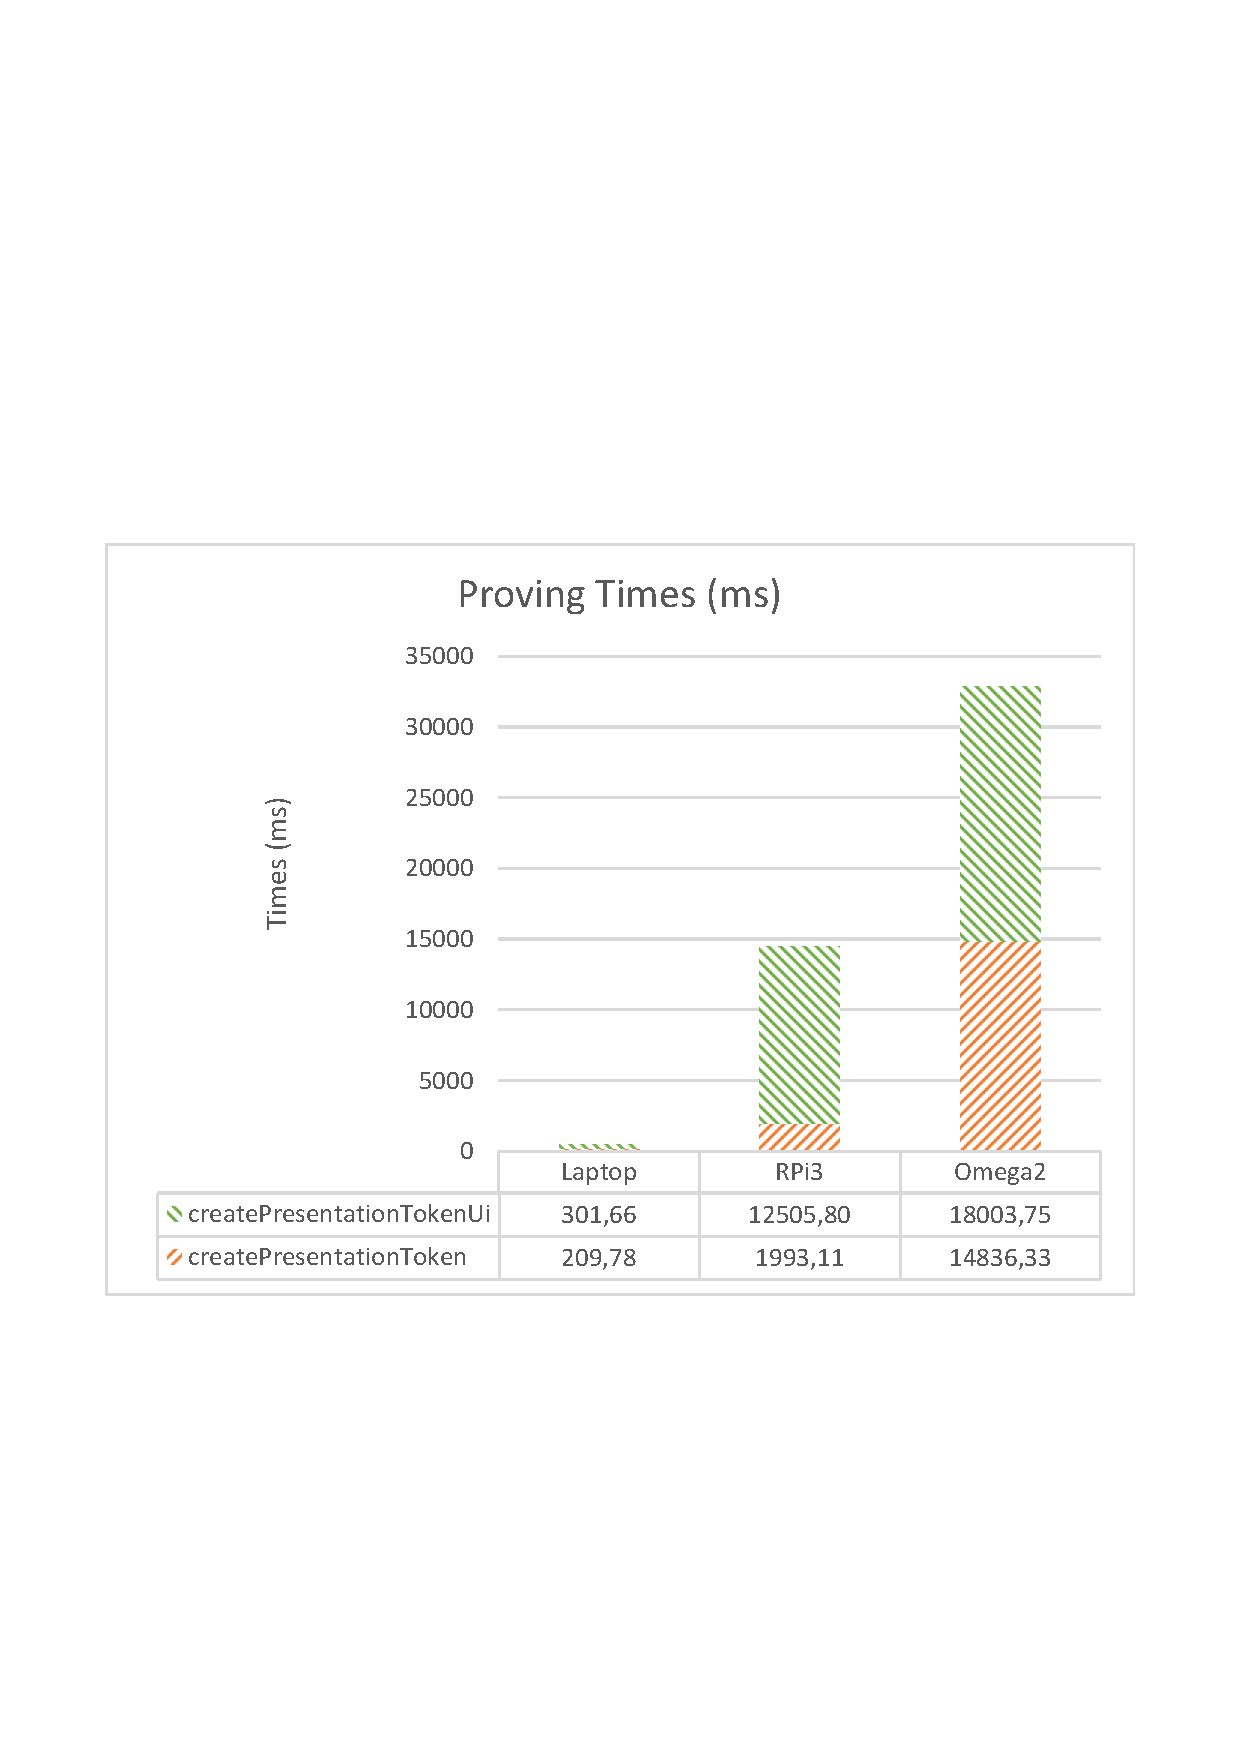
\includegraphics[width=0.8\linewidth]{gfx/graphics/ProvingGraphTable}
	\caption{Proving times (milliseconds)}% and relative speedup.}
	\label{fig:proving:graph}
\end{figure}

%\begin{figure}[bth]
%	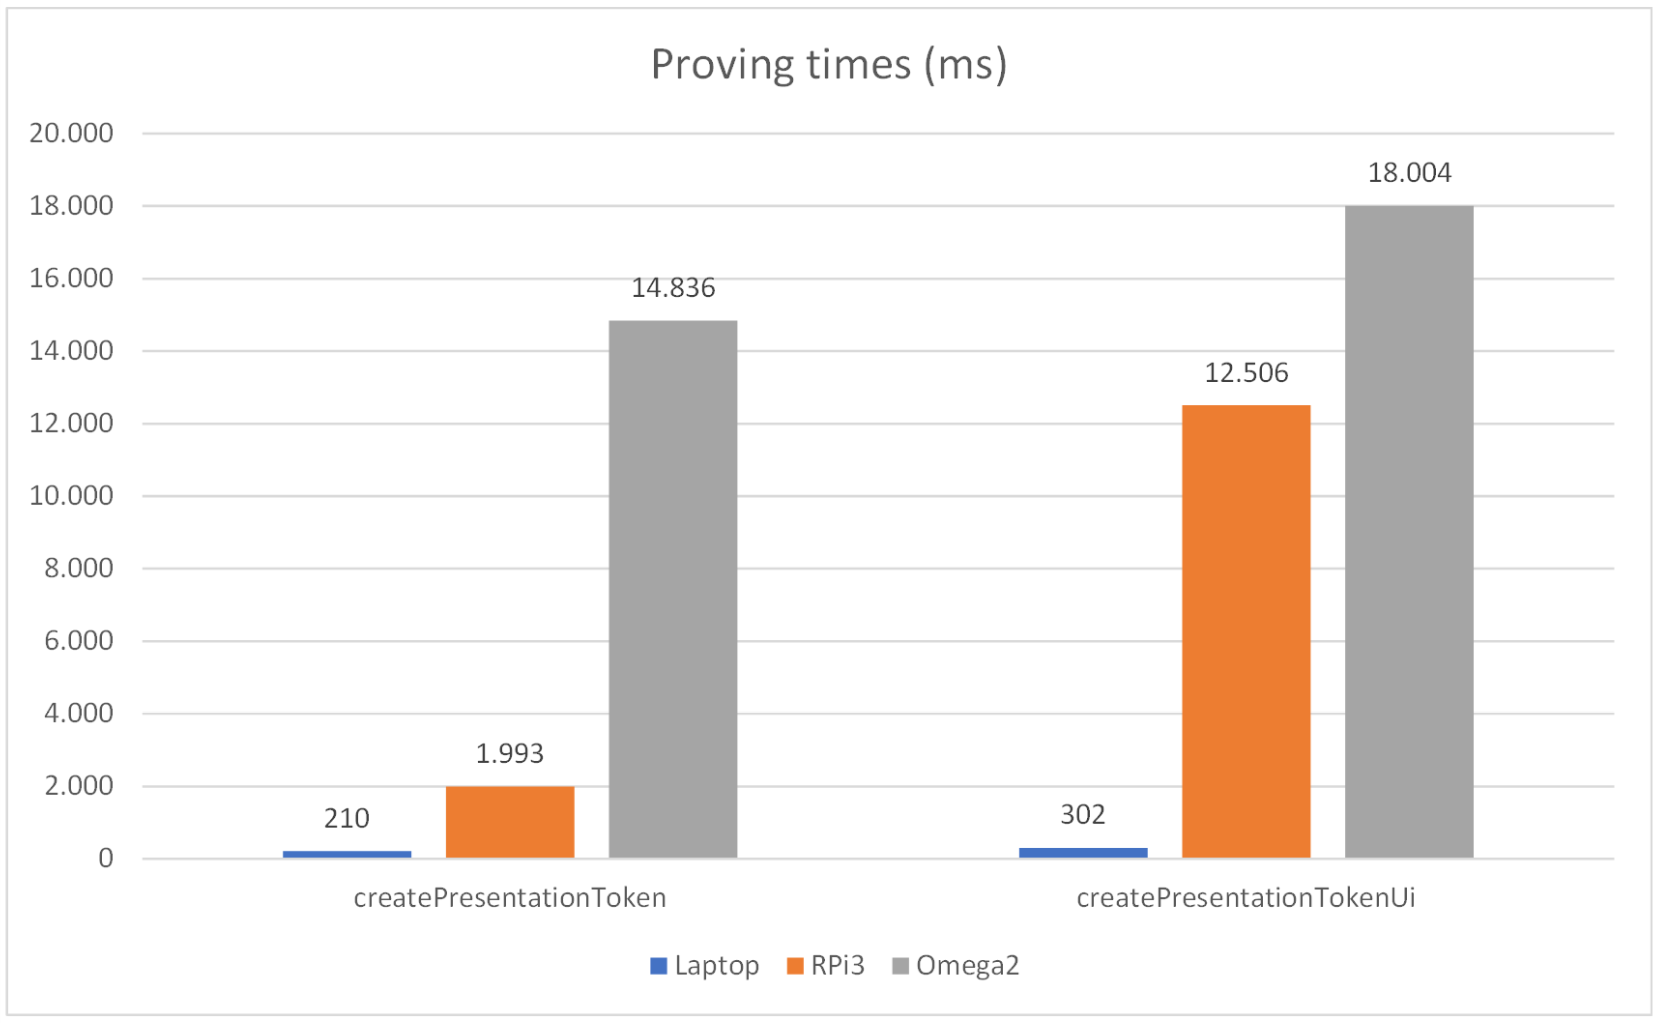
\includegraphics[width=\linewidth]{gfx/graphics/proving}
%	\caption{Proving times (milliseconds). Comparison graph}
%	\label{fig:proving:graph2}
%\end{figure}

Unlike the previous steps, the Proving is the most used method and key feature of the P2ABCE ecosystem. The laptop performs a prove in less than one second, the RPi3 standalone needs $15$ seconds, but the P2ABCE IoT deployment needs almost $15$ seconds for the first step, and $18$s for the second step, $33$ seconds total to generate a Presentation Token.

\hfil

%\paragraph{Memory usage on the Omega2}\hfil

After the tests, in a new series of executions, the tool \texttt{time -v} provided the \texttt{Maximum resident set size (kbytes)} of the PoC IoT smart card, i.e. the maximum size of RAM used by the process since its launch. The mean of the maximum memory usage measured was $6569.6$ kbytes. This includes the use of static memory for all the \textit{global variables} of the smart card logic, as well as the dynamic memory allocated by the external utilities libraries, GMPlib, OpenSSL and cJSON.

GMP and OpenSSL always allocate the data in their own ADT, which involves copying the arrays of bytes representing the big modular integers from the cryptographic operations instead of using the byte array representations of the smart card logic. cJSON, used in the serialization of the smart card, for storage and debugging purposes, stores a copy of every saved variable in a JSON tree structure, then allocates a string with the JSON, that then the user can write to a file.
These multiple poor uses of memory could be avoided in future versions of the PoC, with a custom binary serialization or arithmetic library.


\subsection{Validation conclusions}

% De https://abc4trust.eu/download/D4.2%20Final%20Reference%20Implementation.pdf  página 45 discussion, que si la credencial está cacheada se reducen ciertos tiempos, este es el peor caso

Below, Table~\ref{totaltime} sums up the time used in each step of the test for the IoT scenario.
The first step, \textit{System Setup} is done only once when the system is being deployed, and the \textit{IoT Smart Card Setup} only once per device.
Because a device can have more than one credential, the Issuance step is significant when we issue multiple credentials over the device's lifetime.
Finally, the Proving step is expected to be the most commonly performed operation. The times obtained are in pair with the tests performed in \cite{D42} for their smart card implementation, where the bottleneck is the copy of group parameters and other data from the IoT smart card to the server. The rest of the time is spent mostly with the cryptographic operations. 
The fact that it lasts over half a minute implies that we should not use this PoC for \textit{real-time} applications yet. 
Nevertheless, for many other IoT applications, the fact this operation can be performed multiple times per hour, presents an useful tool for privacy. 


\begin{table}[!ht]
	\centering
	\begin{tabular}{|r|r|r|r|}
		\hline
		System & IoT Smart  & Credential  & Prove Presen-\\
		Setup & Card Setup & Issuance & tation Policy\\ \hline
		3.77 s & 19.19 s & 36.48 s & 32.84 s \\ \hline
	\end{tabular}
	\caption{Total time spent for each step in the Omega2+RPi3 scenario.}
	\label{totaltime}
\end{table}

%\begin{figure}[bth]
%	\begin{center}
%		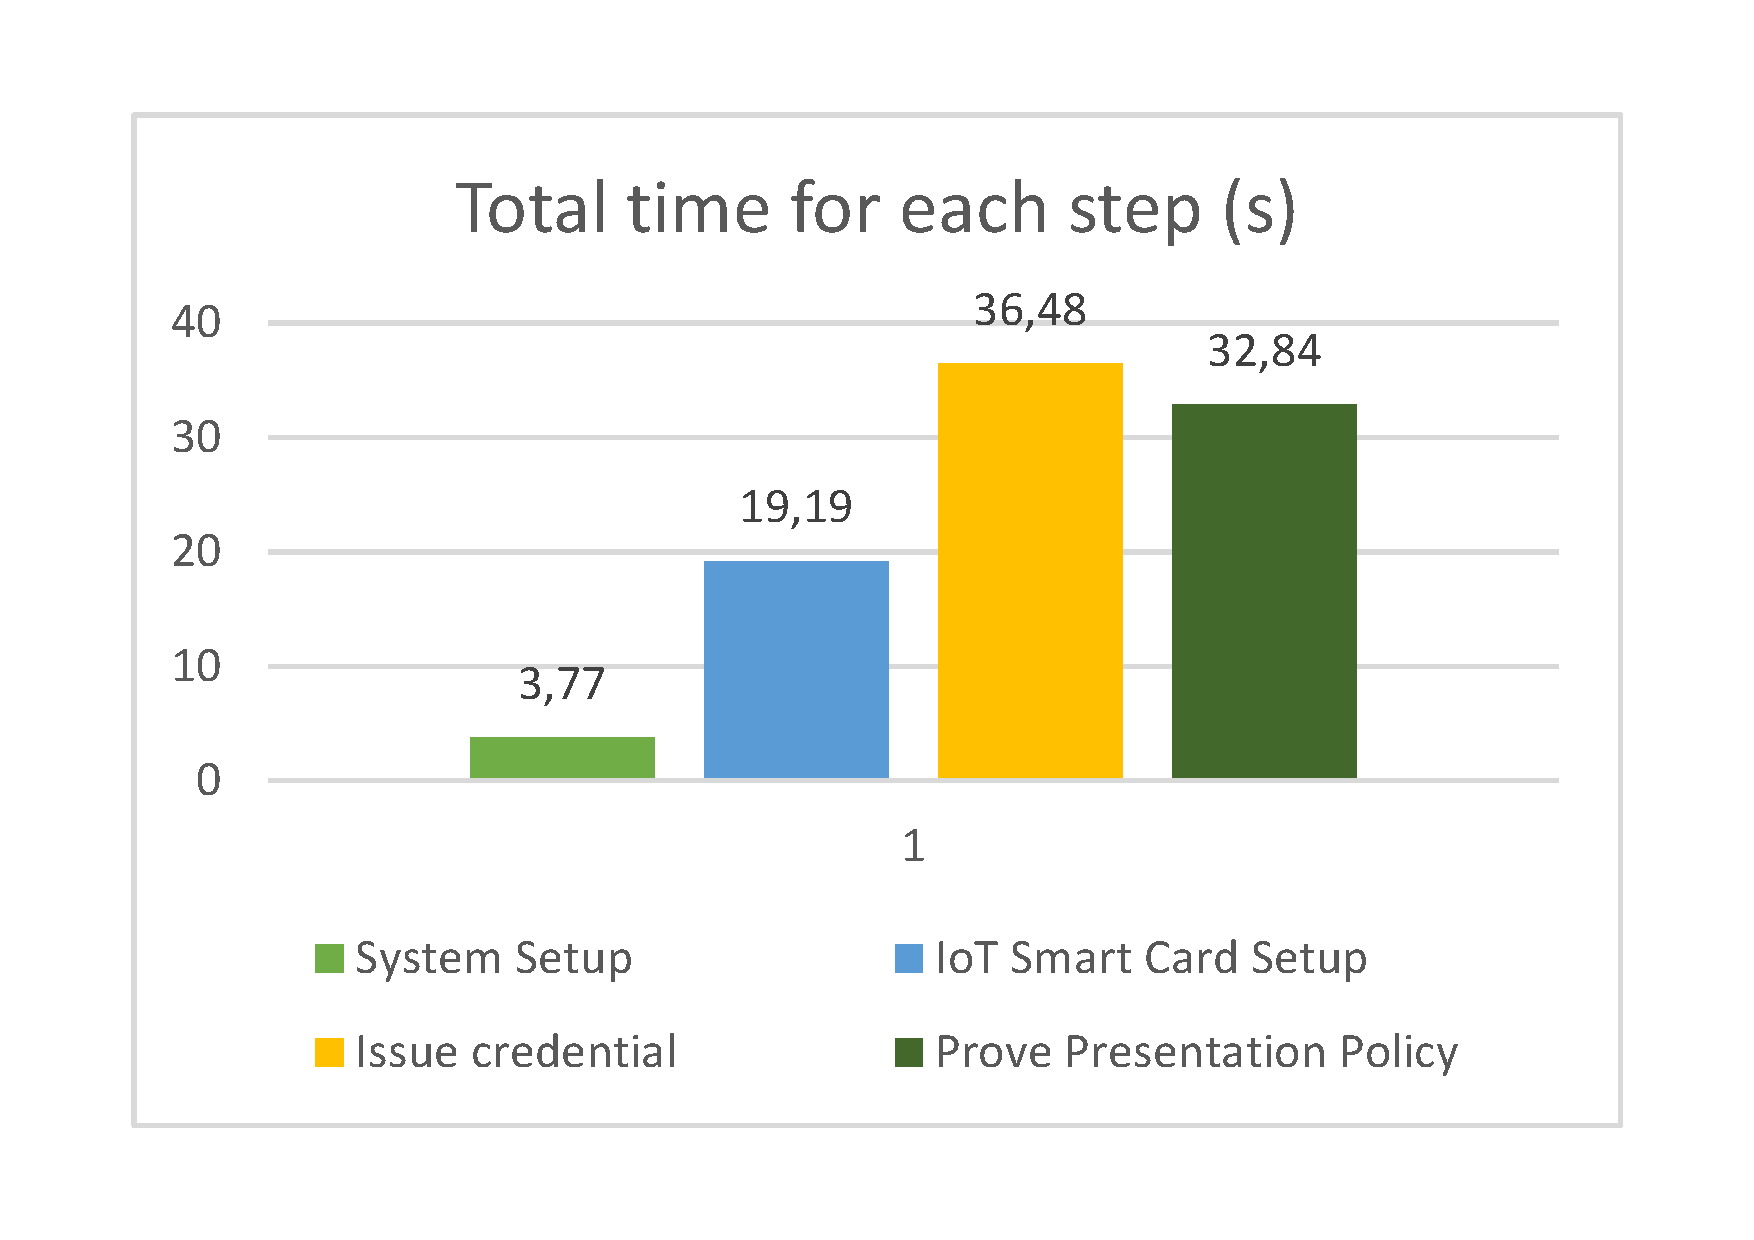
\includegraphics[width=0.75\linewidth]{gfx/graphics/TotalGraph}
%	\end{center}
%	\caption{Total time spent for each step in the Omega2+RPi3 scenario.}
%	\label{totaltime}
%\end{figure}


